\documentclass{article}
\usepackage[left=3cm,right=3cm,
    top=2cm,bottom=2cm,bindingoffset=0cm]{geometry}
\usepackage{graphicx} % Required for inserting images

\usepackage[english, russian]{babel}
\usepackage[T2A]{fontenc}			% кодировка
\usepackage[utf8]{inputenc}			% кодировка исходного текста

\title{\textbf{Лабораторная работа 1.3.1.} \linebreak
ОПРЕДЕЛЕНИЕ МОДУЛЯ ЮНГА}
\author{Попова Софья Б04-401}
\date{October 2024}

\begin{document}

\maketitle

\subsection*{Цель работы}
Экспериментально получить зависимость между напряжением и деформацией (закон Гука) для простейших напряженных состояний упругих тел: одноосного растяжения и чистого изгиба.


\section*{Часть 1: Определение модуля Юнга на основе исследования деформаций растяжения проволоки.}

\subsubsection*{Оборудование}
Прибор Лермантова, проволока из исследуемого материала, лазер закрепленный на шкале, набор грузов, микрометр, двухметровая линейка.


\subsubsection*{Теоретическая часть}

\noindent
Связь между удлиннением проволоки $\Delta$l и силой P, вызывающей это удлинение, выражается законом Гука: 
\begin{equation}\label{нср}
\frac{P}{S}=E\frac{\Delta l}{l}
\end{equation}
где $l$ - начальная длина проволоки, $S$ - ее сечение, $E$ - константа, характеризующая упругие свойства материала (модуль Юнга).

\noindent
Проволока слабо растяжима, следовательно справедлива оценка $\Delta l \ll r$, где $r$ - длина рычага. С учетом этого, угол наклона зеркальца к горизонтали можно найти как $\alpha = \frac{\Delta l}{r}$. С другой стороны, $\alpha = \frac{n}{2h}$, где $n$ - показания шкалы, $h$ - расстояние от шкалы до зеркальца. Таким образом, удлинение проволоки можно выразить как: 
\begin{equation}\label{нср}
\Delta l = n\frac{r}{2h}
\end{equation}


\subsubsection*{Экспериментальная часть}

\textbf{1.}

\noindent
Расстояние до зеркала: $h=150,5\pm 0,5$см ($=1,505\pm 0,005$м)

\noindent
Длина рычага: $r=13$мм ($=0,013$м)

\noindent
\textbf{2.}

\noindent
Диаметр проволоки: $d=0,73$мм ($=0,00078$м)

\noindent
Сечение $S\approx 0,42$ мм $^2$ ($=4,2\cdot10^{-7} $ м $^2$)

\noindent
\textbf{3.}

\noindent
Длина проволоки: $l=178\pm 1$см ($=1,78\pm 0,01$м)

\noindent
\textbf{4.}

\noindent
Максимальная величина нагрузки: $\sigma S=90\cdot0.42=37,8$кг

\noindent
$30\%$ от максимальной величины $=11,34$кг

\noindent
Это меньше макссимальной массы, которую можно получить всеми грузами, значит в ходе эксперимента масса не выйдет за пределы области, где удлинение проволоки пропорционально ее натяжению. Это подтвердилось в ходе экспериментальной проверки (остаточные деформации не наблюдались).

\noindent
\textbf{5.}

\noindent
Расчет $\Delta l$ производим по формуле (2), а погрешность измерения $\Delta l$ оцениваем по формуле: $$\varepsilon_{\Delta l} = \sqrt{(\frac{\sigma_n}{n})^2+(\frac{\sigma_r}{r})^2+(\frac{\sigma_h}{h})^2}$$ где $\frac{\sigma_n}{n}<1\%$, $r$ - дано, $\frac{\sigma_h}{h} = \frac{0,5}{1,505}<1\%$. Значит $\varepsilon_{\Delta l}<1\%$ 

\noindent
Из (1): $E=\frac{Pl}{S\Delta l} = \frac{lg}{S}\cdot\frac{m}{\Delta l} = \frac{124600000}{3}\cdot\frac{m}{\Delta l}$

\begin{table}[!h]
    \centering
    \begin{tabular}{|c|c|c|c|c|}
        \hline
         Количество грузов & Масса грузов $m$, г & Значение шкалы $n$, см  & $\Delta n$, см & $\Delta l$, см \\
         \hline
        0  & 478,7  & 23,9 & -   & -                \\
        1  & 724,4  & 25,4 & 1,5 & 6,5\cdot 10^{-3} \\
        2  & 969,6  & 26,6 & 1,2 & 5,2\cdot 10^{-3} \\
        3  & 1215,2 & 27,9 & 1,3 & 5,6\cdot 10^{-3} \\
        4  & 1460,7 & 29,4 & 1,5 & 6,5\cdot 10^{-3} \\
        5  & 1706,2 & 30,4 & 1   & 4,3\cdot 10^{-3} \\
        6  & 1952,3 & 31,9 & 1,5 & 6,5\cdot 10^{-3} \\
        7  & 2198   & 33,1 & 1,2 & 5,2\cdot 10^{-3} \\
        8  & 2443,6 & 34,3 & 1,2 & 5,2\cdot 10^{-3} \\
        9  & 2689,7 & 35,5 & 1,2 & 5,2\cdot 10^{-3} \\
        10 & 2935,5 & 36,6 & 1,1 & 4,8\cdot 10^{-3} \\
        9  & 2689,7 & 35,5 & 1,1 & 4,8\cdot 10^{-3} \\
        8  & 2443,6 & 34,3 & 1,2 & 5,2\cdot 10^{-3} \\
        7  & 2198   & 33   & 1,3 & 5,6\cdot 10^{-3} \\
        6  & 1952,3 & 31,7 & 1,3 & 5,6\cdot 10^{-3} \\
        5  & 1706,2 & 30,3 & 1,4 & 6\cdot 10^{-3}   \\
        4  & 1460,7 & 28,7 & 1,6 & 6,9\cdot 10^{-3} \\
        3  & 1215,2 & 27,8 & 0,9 & 3,9\cdot 10^{-3} \\
        2  & 969,6  & 26,5 & 1,3 & 5,6\cdot 10^{-3} \\
        1  & 724,4  & 25,3 & 1,2 & 5,6\cdot 10^{-3} \\
        0  & 478,7  & 23,8 & 1,5 & 6,5\cdot 10^{-3} \\
        \hline
    \end{tabular}
\end{table}

\noindent
\textbf{6.}

\noindent
Зависимость $\Delta l$ от $m$ изображена на графиках (рис. 1 и рис. 2)

\noindent
Из полученного графика модуль Юнга определяется по формуле:$$E=\frac{\Delta m}{\Delta l}\cdot\frac{lg}{S} = k\cdot\frac{lg}{S}$$ $E = 1,875\cdot10^{11}$Па

$$\sigma_E = \sqrt{(\frac{\sigma k}{k})^2 + (\frac{\sigma S}{S})^2 + (\frac{\sigma l}{l})^2}$$   
$\sigma_E = \sqrt{(\frac{0,01}{1,78})^2} \approx 0,006 (<1\%)$


\begin{figure}
    \centering
    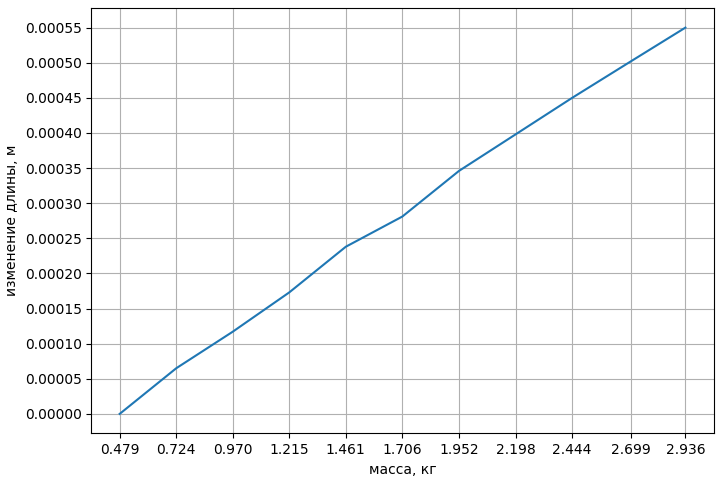
\includegraphics[width=1\linewidth]{проволока возр.png}
    \caption{Возрастающ. нагрузка}
\end{figure}
\begin{figure}
    \centering
    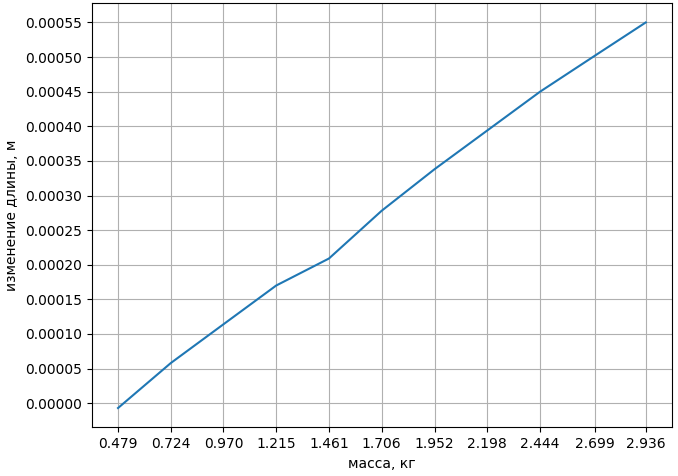
\includegraphics[width=1\linewidth]{проволока убыв.png}
    \caption{Убывающ. нагрузка}
\end{figure}

\subsubsection*{Вывод}
Полученное значение модуля Юнга (187,5 ГПа) отличается от табличного значения модуля Юнга лдя стали и железа (200ГПа) на $\frac{200-187,5}{200} = 0,0625$ $6,25\%$

\newpage
\section*{Часть 2: Определение модуля Юнга по измерениям изгиба балки.}

\subsubsection*{Оборудование}
Стойка для изгибания балки, индикатор для измерения величины прогиба, набор исследуемых балок, грузы, линейка, штангенциркуль.


\subsubsection*{Теоретическая часть}
Модуль Юнга материала стержня $E$ связан с величиной прогиба $y_{max}$ как: 
\begin{equation}\label{нср}
E=\frac{Pl^3}{4ab^3y_{max}}
\end{equation}
 где $P$ - нагрузка на стержень, $l$ - расстояние между точками опоры, $a$ - ширина балки, $b$ - толщина балки.


\subsubsection*{Экспериментальная часть}

\noindent
\textbf{1.}

\noindent
Расстояние $AA' = 50 \pm 0.5$см

\noindent
\textbf{2.}

\noindent
Металлическая балка: 

Ширина = $2,05 \pm0.05$ см  |  Толщина = $0,4 \pm0.05$ см

\noindent
Деревянная балка: 

Ширина = $1,9 \pm0.05$ см  |  Толщина = $1 \pm0.05$ см

\noindent
\textbf{3.}

\noindent
Результаты измерений изгиба металлической балки зафиксированны в таблице 1.

\noindent
\textbf{4.}

\noindent
При смещениии призмы от точки, принятой за середину балки, изменение $\lambda$ не наблюдалось.

\noindent
\textbf{5.}

\noindent
Результаты измерений изгиба перевернутой металлической балки зафиксированны в таблице 2. $\lambda$ увеличилась, что может говорить о меньшем сопротивлении изгибу в этом направлении у балки.

\noindent
\textbf{6.}

\noindent
Результаты измерений изгиба деревянной балки зафиксированны в таблицах 3 и 4.

\noindent
\textbf{7.}

\noindent
По данным из таблиц построими графики зависимости $\lambda$ от веса для повышения и понижения нагрузки.
По наклону графиков определяем средние значения модуля Юнга по формуле (3) и погрешность по формуле: $$\sigma_E = \sqrt{3(\frac{\sigma l}{l})^2 + (\frac{\sigma_{P/\lambda}}{P/\lambda})^2 + (\frac{\sigma a}{a})^2 + 3(\frac{\sigma b}{b})^2}$$

\begin{table}[!h]
    \centering
    \begin{tabular}{|c|c|c}
         \hline
         \multicolumn{3}{|c|}{ Металлическая балка} \\
         \hline
                        & Значение             & $\sigma$ \\
            $P/\lambda$ & 9226,1 Н/м           &    100   \\
                  E     & $2,2\cdot10^{11}$Н/м &    0,61  \\
         \hline
         \multicolumn{3}{|c|}{Деревянная балка} \\
         \hline
                        & Значение              & $\sigma$ \\
            $P/\lambda$ & 7502,6 Н/м            & 100      \\
                 E      & $1,23\cdot10^{11}$Н/м & 0,39     \\
         \hline
    \end{tabular}
\end{table}

\subsubsection*{Вывод}
Полученнные значения модуля Юнга для стали ($E = 2,2\cdot10^{11}$Па) и дерева ($E = 1,23\cdot10^{11}$Па) близки к табличным значениям (для стали: $E\approx2\cdot10^{11}$, для дерева $E$ лежит в пределах 11-15 ГПа в зависимасоти от породы)

\newpage
\subsubsection*{Таблицы и графики}

\begin{table}[!h]
    \centering
    \begin{tabular}{|c|c|c|c|}
        \hline
         Количество грузов & Масса грузов $m$, г & $\lambda$, мм  \\
         \hline
        0  & 105,1  & 0                  \\
        1  & 587,6  & $0,36$  \\
        2  & 1065,8 & $0,98$  \\
        3  & 1533,7 & $1,65$\\
        4  & 2035   & $2,29$ \\
        5  & 2538,1 & $3,00$ \\
        6  & 3041,4 & $3,68$ \\
        7  & 3508,1 & $4,29$ \\
        8  & 4012,6 & $4,96$ \\
        9  & 4474,4 & $5,64$ \\
        10 & 4985,4 & $6,36$ \\
        9  & 4474,4 & $5,77$ \\
        8  & 4012,6 & $5,19$ \\
        7  & 3508,1 & $4,43$ \\
        6  & 3041,4 & $3,80$ \\
        5  & 2538,1 & $3,10$ \\
        4  & 2035   & $2,41$ \\
        3  & 1533,7 & $1,72$ \\
        2  & 1065,8 & $1,08$ \\
        1  & 587,6  & $0,48$  \\
        0  & 105,1  & 0                 \\
        \hline
    \end{tabular}
    \caption{Металлическая балка. Измерение 1}
\end{table}

\begin{table}[!h]
    \centering
    \begin{tabular}{|c|c|c|c|}
        \hline
         Количество грузов & Масса грузов $m$, г & $\lambda$, мм \\
         \hline
        0  & 105,1  & 0                 \\
        1  & 587,6  & $0.67$  \\
        2  & 1090,7 & $1.35$ \\
        3  & 1568,9 & $2.00$ \\
        4  & 2036,8 & $2.60$ \\
        5  & 2538,1 & $3.33$ \\
        6  & 3041,4 & $4.01$ \\
        7  & 3508,1 & $4.61$ \\
        8  & 4012,6 & $5.32$ \\
        9  & 4474,4 & $6.00$ \\
        10 & 4985,4 & $6.80$ \\
        9  & 4474,4 & $6.04$ \\
        8  & 4012,6 & $5.50$ \\
        7  & 3508,1 & $4.82$ \\
        6  & 3041,4 & $4.17$ \\
        5  & 2538,1 & $3.50$ \\
        4  & 2036,8 & $2.80$ \\
        3  & 1568,9 & $2.16$ \\
        2  & 1090,7 & $1.53$ \\
        1  & 587,6  & $0.82$  \\
        0  & 105,1  & $0.13$  \\
        \hline
    \end{tabular}
    \caption{Металлическая балка. Измерение 2}
\end{table}

\begin{table}[!t]
    \centering
    \begin{tabular}{|c|c|c|c|}
        \hline
         Количество грузов & Масса грузов $m$, г & $\lambda$, мм  \\
         \hline
        0  & 105,1  & 0                 \\
        1  & 587,6  & $0.54$  \\
        2  & 1090,7 & $1.32$ \\
        3  & 1558,6 & $1.96$ \\
        4  & 2025,3 & $2.70$ \\
        5  & 2487,1 & $3.44$ \\
        6  & 2998,7 & $4.24$ \\
        7  & 3502,6 & $5.02$ \\
        8  & 4005,9 & $5.78$ \\
        9  & 4484,1 & $6.58$ \\
        10 & 4985,4 & $7.19$ \\
        9  & 4484,1 & $6.43$ \\
        8  & 4005,9 & $5.73$ \\
        7  & 3502,6 & $4.96$ \\
        6  & 2998,7 & $4.23$ \\
        5  & 2487,1 & $3.43$ \\
        4  & 2025,3 & $2.71$ \\
        3  & 1558,6 & $2.08$ \\
        2  & 1090,7 & $1.32$ \\
        1  & 587,6  & $0.55$  \\
        0  & 105,1  & 0                 \\
        \hline
    \end{tabular}
    \caption{Деревянная балка. Измерение 1}
\end{table}

\begin{table}[!h]
    \centering
    \begin{tabular}{|c|c|c|c|}
        \hline
         Количество грузов & Масса грузов $m$, г & $\lambda$, мм \\
         \hline
        0  & 105,1  & 0                 \\
        1  & 587,6  & $0.69$  \\
        2  & 1054,3 & $1.42$ \\
        3  & 1557,4 & $2.15$ \\
        4  & 2019,2 & $2.90$ \\
        5  & 2487,1 & $3.60$ \\
        6  & 2998,1 & $4.39$ \\
        7  & 3501,4 & $5.17$ \\
        8  & 4005,9 & $5.95$ \\
        9  & 4484,1 & $6.67$ \\
        10 & 4985,4 & $7.43$ \\
        9  & 4484,1 & $6.90$ \\
        8  & 4005,9 & $6.12$ \\
        7  & 3501,4 & $5.33$ \\
        6  & 2998,1 & $4.54$ \\
        5  & 2487,1 & $3.74$ \\
        4  & 2019,2 & $3.03$ \\
        3  & 1557,4 & $2.32$ \\
        2  & 1054,3 & $1.55$ \\
        1  & 587,6  & $0.84$ \\
        0  & 105,1  & $0.07$ \\
        \hline
    \end{tabular}
    \caption{Деревянная балка. Измерение 2}
\end{table}

\newpage

\begin{figure}
    \centering
    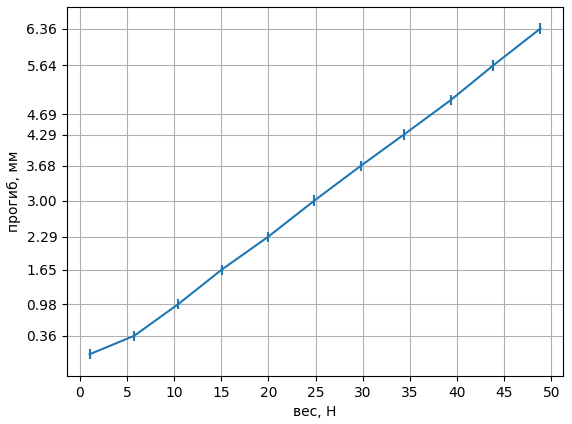
\includegraphics[width=0.9\linewidth]{металл 1 возраст.png}
    \caption{Металлическая балка. Измерение 1. Повышение нагрузки.}
    \label{fig:enter-label}
\end{figure}

\begin{figure}
    \centering
    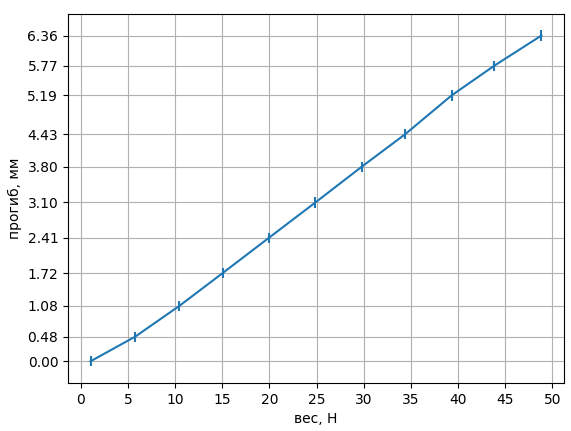
\includegraphics[width=0.9\linewidth]{металл 1 убыв.png}
    \caption{Металлическая балка. Измерение 1. Понижение нагрузки.}
    \label{fig:enter-label}
\end{figure}

\begin{figure}
    \centering
    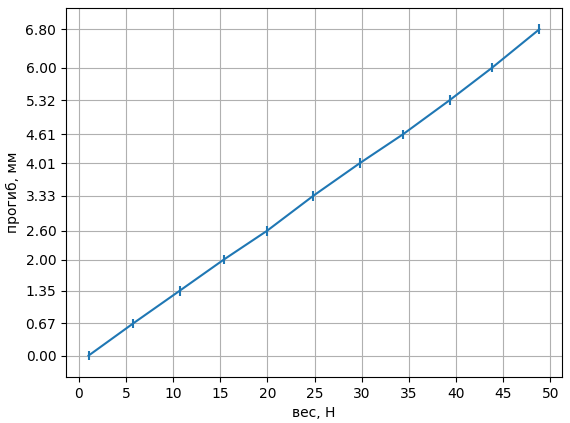
\includegraphics[width=0.9\linewidth]{металл 2 возраст.png}
    \caption{Металлическая балка. Измерение 2. Повышение нагрузки.}
    \label{fig:enter-label}
\end{figure}

\begin{figure}
    \centering
    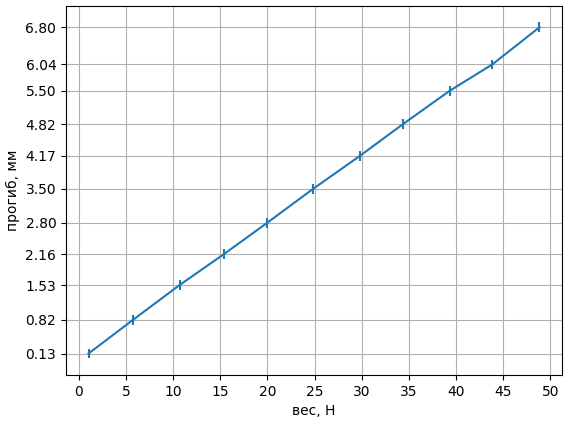
\includegraphics[width=0.9\linewidth]{металл 2 убыв.png}
    \caption{Металлическая балка. Измерение 2. Понижение нагрузки.}
    \label{fig:enter-label}
\end{figure}


\begin{figure}
    \centering
    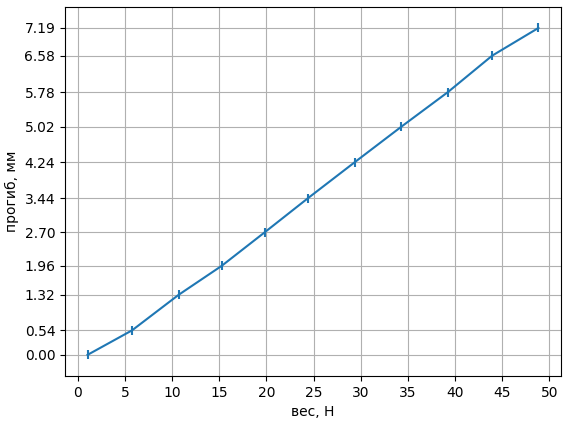
\includegraphics[width=0.9\linewidth]{дерево 1 возраст.png}
    \caption{Деревянная балка. Измерение 1. Повышение нагрузки.}
    \label{fig:enter-label}
\end{figure}

\begin{figure}
    \centering
    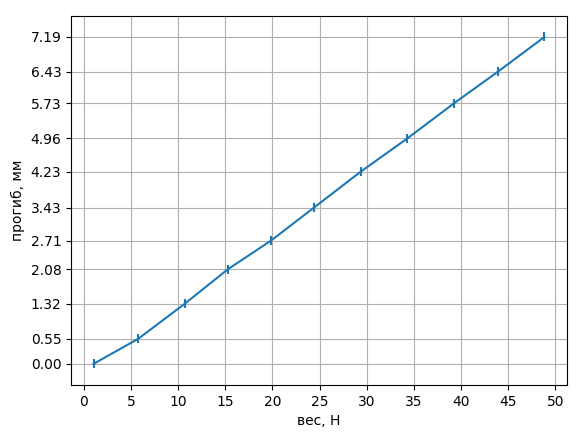
\includegraphics[width=0.9\linewidth]{дерево 1 убыв.png}
    \caption{Деревянная балка. Измерение 1. Понижение нагрузки.}
    \label{fig:enter-label}
\end{figure}

\begin{figure}
    \centering
    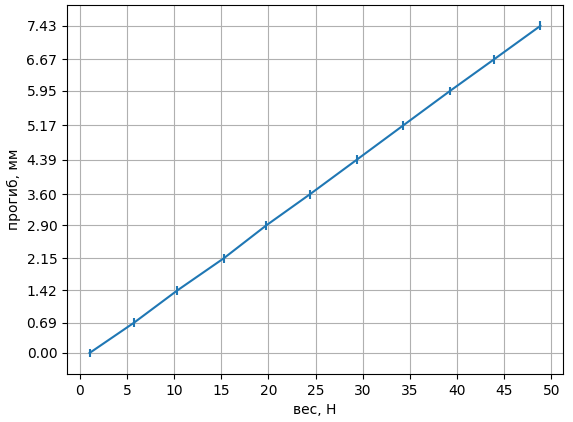
\includegraphics[width=0.9\linewidth]{дерево 2 возраст.png}
    \caption{Деревянная балка. Измерение 2. Повышение нагрузки.}
    \label{fig:enter-label}
\end{figure}

\begin{figure}
    \centering
    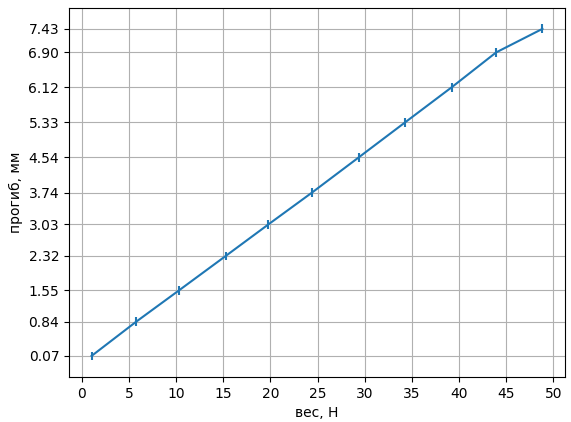
\includegraphics[width=0.9\linewidth]{дерево 2 убыв.png}
    \caption{Деревянная балка. Измерение 2. Понижение нагрузки.}
    \label{fig:enter-label}
\end{figure}


\end{document}

